\section{Auswertung}
\label{sec:Auswertung}

%Siehe \autoref{fig:plot}!
\subsection{Kontrast}

Die zur Bestimmung des Kontrasts gemessene maximale und minimale Intensität bzw. Spannung in Abhängigkeit des Polaristionswinkels $\phi$ ist in \autoref{tab:kontrast} aufgeführt.
Daraus lässt sich über \autoref{eq:kontrast1} der Kontrast für jede Winkeleinstellung berechnen. 
\begin{table}
    \centering
    \caption{Winkeleinstellung des Polaristionsfilters $\phi$ und die entsprechenden maximalen und minimalen Spannungen an der Photodiode. Der Kontrast $K$ des Interferometers ergibt sich aus den Intensitäten.}
    \label{tab:kontrast}
    \begin{tabular}{c c c c}
        \toprule
        $\phi \,/\, \unit{\degree}$ & $I_\text{min} \,/\, \unit{\volt}$ & $I_\text{max} \,/\, \unit{\volt}$ & $K$ \\
        \midrule
        $0  $ &   $ 0.80\pm 0.01$ & $ 	0.99 \pm 0.01$ &  $ 0.11 \pm 0.01 $ \\
        $15	$ &   $ 0.48\pm 0.01$ & $	0.82 \pm 0.01$ &  $ 0.26 \pm 0.01 $ \\
        $30	$ &   $ 0.13\pm 0.01$ & $	0.77 \pm 0.01$ &  $ 0.71 \pm 0.02 $ \\
        $45	$ &   $ 0.10\pm 0.01$ & $	0.74 \pm 0.01$ &  $ 0.76 \pm 0.02 $ \\
        $50	$ &   $ 0.06\pm 0.01$ & $	0.84 \pm 0.01$ &  $ 0.87 \pm 0.02 $ \\
        $55	$ &   $ 0.04\pm 0.01$ & $	0.91 \pm 0.01$ &  $ 0.91 \pm 0.02 $ \\
        $60	$ &   $ 0.05\pm 0.01$ & $	0.97 \pm 0.01$ &  $ 0.90 \pm 0.02 $ \\
        $65	$ &   $ 0.09\pm 0.01$ & $	1.07 \pm 0.01$ &  $ 0.84 \pm 0.02 $ \\
        $80	$ &   $ 0.43\pm 0.01$ & $	1.20 \pm 0.01$ &  $ 0.47 \pm 0.01 $ \\
        $95	$ &   $ 0.92\pm 0.01$ & $	1.22 \pm 0.01$ &  $ 0.14 \pm 0.01 $ \\
        $110$ &   $ 0.54\pm 0.01$ & $  	1.95 \pm 0.01$ &  $ 0.57 \pm 0.01 $ \\
        $125$ &   $ 0.20\pm 0.01$ & $  	2.85 \pm 0.01$ &  $ 0.87 \pm 0.01 $ \\
        $130$ &   $ 0.15\pm 0.01$ & $  	3.00 \pm 0.01$ &  $ 0.90 \pm 0.01 $ \\
        $135$ &   $ 0.14\pm 0.01$ & $  	2.80 \pm 0.01$ &  $ 0.90 \pm 0.01 $ \\
        $140$ &   $ 0.14\pm 0.01$ & $  	2.89 \pm 0.01$ &  $ 0.91 \pm 0.01 $ \\
        $145$ &   $ 0.23\pm 0.01$ & $  	2.55 \pm 0.01$ &  $ 0.83 \pm 0.01 $ \\
        $160$ &   $ 0.56\pm 0.01$ & $  	2.16 \pm 0.01$ &  $ 0.59 \pm 0.01 $ \\
        $170$ &   $ 0.78\pm 0.01$ & $  	1.54 \pm 0.01$ &  $ 0.32 \pm 0.01 $ \\
        $180$ &   $ 0.81\pm 0.01$ & $  	1.01 \pm 0.01$ &  $ 0.11 \pm 0.01 $ \\
        \bottomrule
    \end{tabular}
\end{table}
Durch die Messwerte wird ein Fit der Form 
\begin{equation*}
    K(\phi) = A \cdot |\sin{\phi} \cdot \cos{\phi}|
\end{equation*}
gelegt.
Der Fit-Parameter $A$ wird auf
\begin{equation*}
    A = \qty{1.823(501)}{}
\end{equation*}
bestimmt und der entsprechende Fit ist in \autoref{fig:kontrast} dargestellt.
\begin{figure}
    \centering
    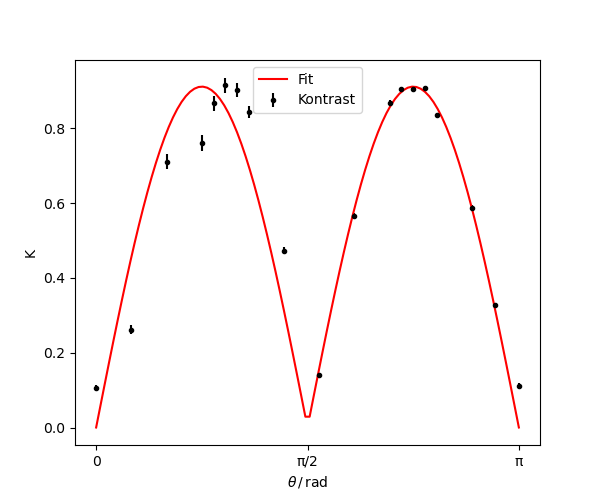
\includegraphics[width=0.9\textwidth]{python/kontrast.png}
    \caption{Der experimentell bestimmte Kontrast mit Ausgleichsfunktion in Abhängigkeit des Polarisationswinkels $\phi$.}
    \label{fig:kontrast}
\end{figure}
\FloatBarrier

\subsection{Brechungsindex von Glas}
Die Anzahl der Interferenzmaxima $M$ bei Drehung des Doppelglases von \qty{0}{\degree} bis \qty{10}{\degree} wird 10 mal gemessen.
Für jedes $M$ wird über \autoref{eq:n_glas} der Brechungsindex $n_\text{Glas}$ berechnet.
Das Ergebnis dieser Messreihen ist in \autoref{tab:glas} aufgeführt.
\begin{table}
    \centering
    \caption{Anzahl gemessener Maxima $M$ und der daraus berechnete Brechungsindex $n_\text{Glas}$.}
    \label{tab:glas}
    \begin{tabular}{c c}
        \toprule
        $M$ & $n_\text{Glas}$ \\
        \midrule
        $32 \pm 1 $ & $1.498 \pm 0.023 $ \\
        $35 \pm 1 $ & $1.571 \pm 0.026 $ \\
        $33 \pm 1 $ & $1.522 \pm 0.024 $ \\
        $37 \pm 1 $ & $1.625 \pm 0.027 $ \\
        $32 \pm 1 $ & $1.498 \pm 0.023 $ \\
        $38 \pm 1 $ & $1.652 \pm 0.028 $ \\
        $29 \pm 1 $ & $1.431 \pm 0.021 $ \\
        $36 \pm 1 $ & $1.598 \pm 0.027 $ \\
        $34 \pm 1 $ & $1.546 \pm 0.025 $ \\
        $34 \pm 1 $ & $1.546 \pm 0.025 $ \\
        \bottomrule
    \end{tabular}
\end{table}
Über die Brechungsindizes wird gemittelt und der Brechungsindex von Glas kann auf
\begin{equation*}
    n_\text{Glas} = \qty{1.549(8)}{}.
\end{equation*}
bestimmt werden.
\FloatBarrier

\subsection{Brechungsindex von Luft}
In drei voneinander unabhängigen Messreihen wird die Anzahl der Interferenzmaxima $M$ in Abhängigkeit des Drucks $p$ bestimmt.
Über \autoref{eq:n_luft} wird der Brechungsindex für jeden Messpunkt ermittelt.
Die Ergebnisse sind in \autoref{tab:brechung} aufgelistet.
\begin{table}
    \centering
    \caption{Brechungsindex $n$ in Abhängigkeit des Drucks $p$ in der Gaskammer und der Anzahl der Nulldurchgänge $M$ für drei Durchläufe.}
    \label{tab:brechung}
    \begin{tabular}{r r r r r r r}
        \toprule
        $p \,/\, \unit{\milli\pascal}$ & $M_1$ & $n_1$ & $M_2$ & $n_2$ & $M_3$ & $n_3$ \\
        \midrule
        $50	    $ & $ 3.0\pm1.0	$ & $   1.000019$ & $ 	2.0\pm1.0 $ & $	1.000013$ & $	2.0\pm1.0	$ & $1.000013$ \\
    	$100	$ & $ 5.0\pm1.0	$ & $   1.000032$ & $ 	4.0\pm1.0 $ & $	1.000025$ & $	4.0\pm1.0	$ & $1.000025$ \\
    	$150	$ & $ 7.0\pm1.0	$ & $   1.000044$ & $ 	6.0\pm1.0 $ & $	1.000038$ & $	6.0\pm1.0	$ & $1.000038$ \\
    	$200	$ & $ 9.0\pm1.0	$ & $   1.000057$ & $ 	9.0\pm1.0 $ & $	1.000057$ & $	8.0\pm1.0	$ & $1.000051$ \\
    	$250	$ & $ 11.0\pm1.0$ & $	1.000070$ & $ 	11.0\pm1.0$ & $	1.000070$ & $	11.0\pm1.0	$ & $1.000070$ \\
    	$300	$ & $ 13.0\pm1.0$ & $	1.000082$ & $ 	13.0\pm1.0$ & $	1.000082$ & $	13.0\pm1.0	$ & $1.000082$ \\
    	$350	$ & $ 15.0\pm1.0$ & $	1.000095$ & $ 	15.0\pm1.0$ & $	1.000095$ & $	15.0\pm1.0	$ & $1.000095$ \\
    	$400	$ & $ 17.0\pm1.0$ & $	1.000108$ & $ 	17.0\pm1.0$ & $	1.000108$ & $	17.0\pm1.0	$ & $1.000108$ \\
    	$450	$ & $ 19.0\pm1.0$ & $	1.000120$ & $ 	19.0\pm1.0$ & $	1.000120$ & $	19.0\pm1.0	$ & $1.000120$ \\
    	$500	$ & $ 21.0\pm1.0$ & $	1.000133$ & $ 	21.0\pm1.0$ & $	1.000133$ & $	21.0\pm1.0	$ & $1.000133$ \\
    	$550	$ & $ 23.0\pm1.0$ & $	1.000146$ & $ 	23.0\pm1.0$ & $	1.000146$ & $	23.0\pm1.0	$ & $1.000146$ \\
    	$600	$ & $ 25.0\pm1.0$ & $	1.000158$ & $ 	25.0\pm1.0$ & $	1.000158$ & $	25.0\pm1.0	$ & $1.000158$ \\
    	$650	$ & $ 27.0\pm1.0$ & $	1.000171$ & $ 	27.0\pm1.0$ & $	1.000171$ & $	27.0\pm1.0	$ & $1.000171$ \\
    	$700	$ & $ 30.0\pm1.0$ & $	1.000190$ & $ 	30.0\pm1.0$ & $	1.000190$ & $	30.0\pm1.0	$ & $1.000190$ \\
    	$750	$ & $ 32.0\pm1.0$ & $	1.000203$ & $ 	32.0\pm1.0$ & $	1.000203$ & $	32.0\pm1.0	$ & $1.000203$ \\
    	$800	$ & $ 34.0\pm1.0$ & $	1.000215$ & $ 	34.0\pm1.0$ & $	1.000215$ & $	34.0\pm1.0	$ & $1.000215$ \\
    	$850	$ & $ 36.0\pm1.0$ & $	1.000228$ & $ 	36.0\pm1.0$ & $	1.000228$ & $	36.0\pm1.0	$ & $1.000228$ \\
    	$900	$ & $ 38.0\pm1.0$ & $	1.000241$ & $ 	39.0\pm1.0$ & $	1.000247$ & $	38.0\pm1.0	$ & $1.000241$ \\
    	$950	$ & $ 41.0\pm1.0$ & $	1.000260$ & $ 	41.0\pm1.0$ & $	1.000260$ & $	41.0\pm1.0	$ & $1.000260$ \\
    	$1000	$ & $ 42.0\pm1.0$ & $	1.000266$ & $ 	42.0\pm1.0$ & $	1.000266$ & $	42.0\pm1.0	$ & $1.000266$ \\
        \bottomrule
    \end{tabular}
\end{table}
Für jeden der drei Messreihen wird entsprechend \autoref{eq:n_luft_lorentz} ein Fit der Form
\begin{equation*}
    n(p) = a \cdot \frac{p}{T R} + b 
\end{equation*}
durchgeführt.
Dabei ist $T = \qty{293.05}{\kelvin}$ die vorherrschende Raumtemperatur und $R$ die allgemeine Gaskonstante.
Die ermittelten Parameter sind 
\begin{align*}
    a_1 &= \qty{642(12)e-8}{\cubic\meter\per\mole} & b_1 &= \qty{1.0000035(29)}{} \\
    a_2 &= \qty{657(12)e-8}{\cubic\meter\per\mole} & b_2 &= \qty{0.9999995(29)}{} \\
    a_3 &= \qty{657(12)e-8}{\cubic\meter\per\mole} & b_3 &= \qty{0.9999990(29)}{}.
\end{align*}
Die entsprechenden Fits sind in \autoref{fig:luft} dargestellt.
\begin{figure}
    \centering
    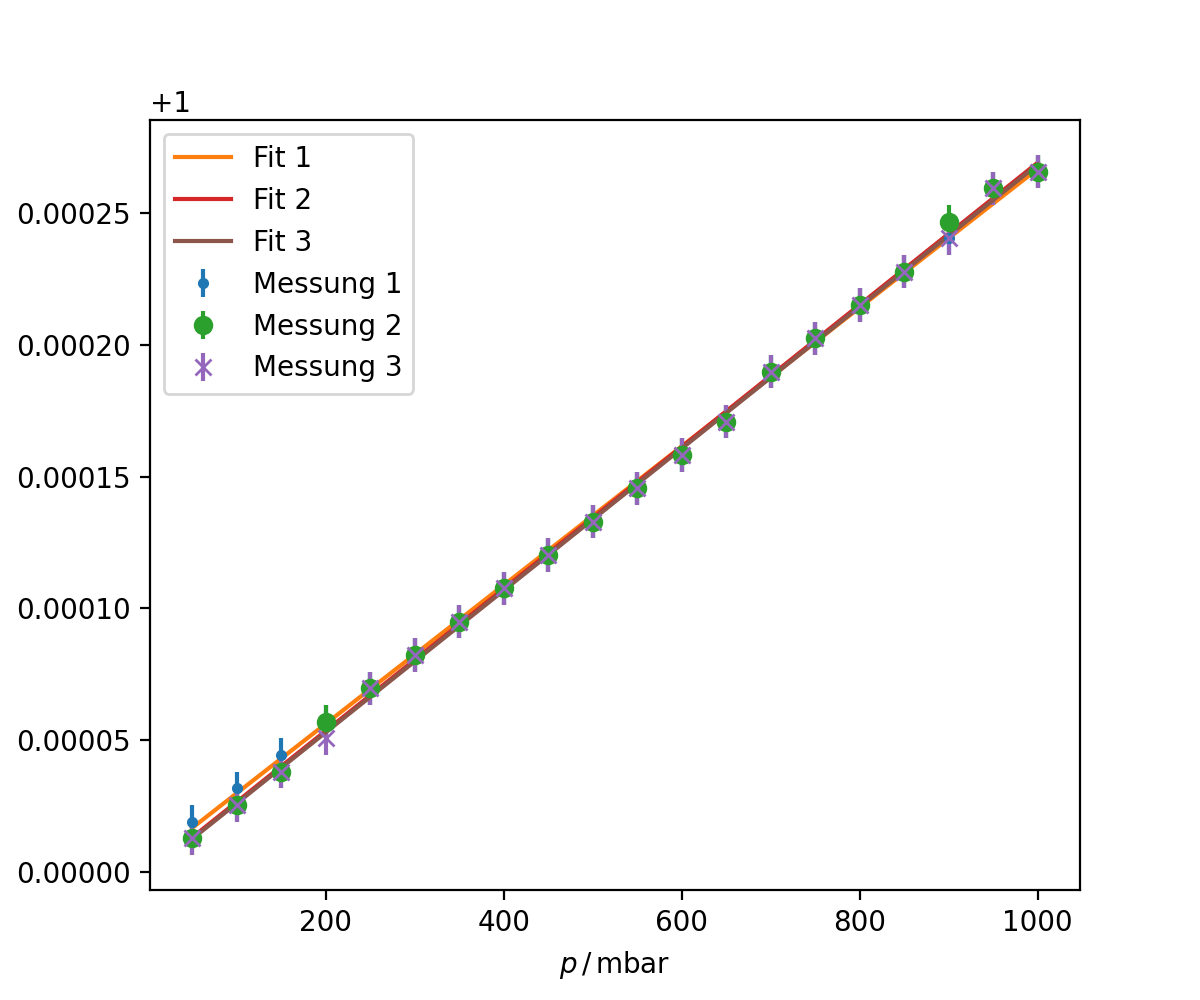
\includegraphics[width=0.9\textwidth]{python/index.png}
    \caption{Brechungsindizes in Abhängigkeit des Luftdrucks in drei verschiedenen Messreihen.}
    \label{fig:luft}
\end{figure}
Der Brechungsindex wird zudem über das Lorentz-Lorenz-Gesetz bei Normatmosphäre berechnet.
Für jede Messreihe werden die Parameter $a$ und $b$ zusammen mit den der Normatmosphäre definierenden Eigenschaften ($T_0 = \qty{288.15}{\kelvin}$ und $p_0 = \qty{1013}{\milli\bar}$) in \autoref{eq:n_luft_lorentz} eingesetzt.
Somit ergibt sich für die Brechungsindizes der einzelnen Messreihen
\begin{align*}
    n_1 &= \qty{1.000275(6)}{} \\
    n_2 &= \qty{1.000277(6)}{} \\
    n_3 &= \qty{1.000277(6)}{}.
\end{align*}
Im Mittel folgt für den Brechungsindex von Luft
\begin{equation*}
    n_\text{Luft} = \qty{1.0002764(34)}{}.
\end{equation*}